\section{Summarising the Posterior Distribution}
The posterior is too much information. We need to summarise it. This is mostly
because, as mere mortals, we might want to communicate our results as a short,
easily remembered ``sound-bite''. For example, say you were trying to estimate
a parameter, and a colleague asked you to state your uncertainty about the
parameter. Well, your posterior distribution might be complicated, it might
have bumps and wiggles in it, or some other kind of structure.
Figure~\ref{fig:complicated_posterior} shows an example of what a complicated
posterior distribution might look like.
\begin{figure}[h!]
\begin{center}
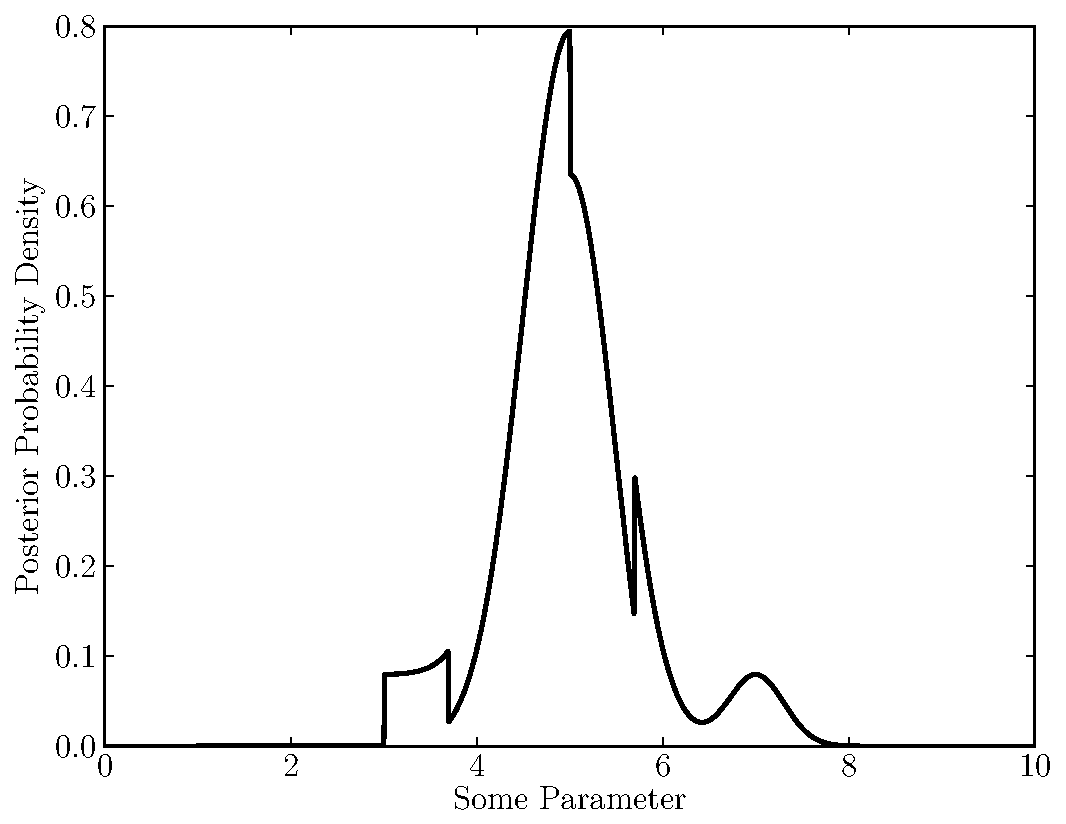
\includegraphics[scale=0.6]{Figures/complicated_posterior.pdf}
\caption{A complicated posterior distribution.\label{fig:complicated_posterior}}
\end{center}
\end{figure}

\subsection{Point Estimates}


\subsection{Credible Intervals}



